\documentclass{standalone}
\usepackage{tikz}
\usepackage{tkz-fct}
\usepackage{tkz-euclide}

\begin{document}


      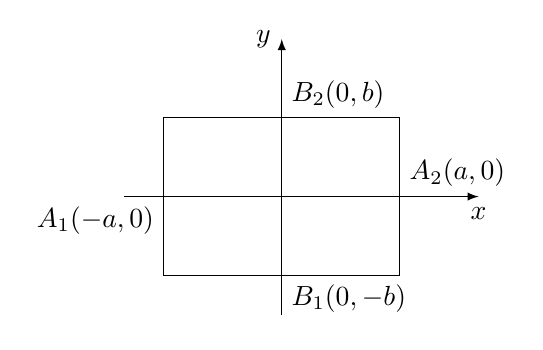
\begin{tikzpicture}
        \tkzInit[xmin=-2,xmax=2,ymin=-1.5,ymax=1.5]
        \tkzDrawXY[noticks]
        %def points
        \tkzDefPoint(-1,0){F1}
        \tkzDefPoint(1,0){F2}
        \tkzDefPoint(-1.5,-1){E}
        \tkzDefPoint(1.5,1){G}
        %draw rectangle
        \draw (E) rectangle (G);
        %%label points
        \node[below left] at (-1.5,0) {$A_1(-a,0)$};
        \node[above right] at (1.5,0) {$A_2(a,0)$};
        \node[below right] at (0,-1) {$B_1(0,-b)$};
        \node[above right] at (0,1) {$B_2(0,b)$};
        %%draw function
        \tkzFctPar[domain=0:2*pi]{(1.5*cos(t))}{(1*sin(t))}
      \end{tikzpicture}


\end{document}
